\documentclass{report}

\usepackage[utf8]{inputenc}
\usepackage{lipsum}%% a garbage package you don't need except to create examples.
\usepackage{fancyhdr}
\usepackage{graphicx}
\usepackage{listings}
\usepackage[dvipsnames]{xcolor}
\usepackage{sectsty}
\chapterfont{\color{BrickRed}}  % sets colour of chapters
\sectionfont{\color{BlueViolet}}  % sets colour of sections
\subsectionfont{\color{OliveGreen}}  % sets colour of sections


\renewcommand{\familydefault}{\sfdefault}
 
\colorlet{punct}{red!60!black}
\definecolor{background}{HTML}{EEEEEE}
\definecolor{delim}{RGB}{20,105,176}
\colorlet{numb}{magenta!60!black}

\lstdefinelanguage{json}{
    basicstyle=\scriptsize\ttfamily,
    numberstyle=\scriptsize,
    stepnumber=1,
    showstringspaces=false,
    breaklines=true,
    backgroundcolor=\color{background},
    literate=
      {:}{{{\color{punct}{:}}}}{1}
      {,}{{{\color{punct}{,}}}}{1}
      {\{}{{{\color{delim}{\{}}}}{1}
      {\}}{{{\color{delim}{\}}}}}{1}
      {[}{{{\color{delim}{[}}}}{1}
      {]}{{{\color{delim}{]}}}}{1},
}

 

% Headers and footers
\pagestyle{fancy}
\lhead{
\includegraphics[width=2cm]{figures/jaqpot_quattro_logo.png}}
%\cfoot{\thepage}
\renewcommand{\headrulewidth}{0.4pt}

\setlength{\headheight}{55pt}


\renewcommand{\sectionmark}[1]{\markright{#1}}
\fancyhf{}
\rhead{\fancyplain{}{JAQPOT Quattro Design}}
\lhead{\fancyplain{}{\rightmark }} 
\cfoot{\fancyplain{}{\thepage}}

\author{kinkyDesign}
\title{
\includegraphics[width=10cm]{figures/jaqpot_quattro_logo.png}\\ 
{\small \texttt{Design principles of jaqpot quattro}}}

\begin{document}


\maketitle

\tableofcontents


%Schemaless schema 
\chapter{Data Model}

%Entities
\section{Entities and their Relationships}

The first step for the development of the new JAQPOT Quattro
platform is to savy the essential entities of the project
and their relationships.
The ER sketch of JAQPOT Quattro is inspirited by the OpenTox
ontology and is concisely presented in the next figure.

\subsection{User}
JAQPOT stores some very basic information about users so as to
manage users' quota. Users have identifying information such as 
their email and name, and a list of limitations (if any) such 
as the maximum number of parallel tasks they can run on the system,
the maximum number of models they may store, datasets to create and
so on.

\subsection{Task and Error Report}
A task is identified by its ID. It has a status (running, queued,
cancelled, etc), percentage of completion, duration to complete (when
it has completed), URI of the result, corresponding HTTP status, 
and also points to the User who created it in the first place, 
as well as a creation timestamp. In case of an exceptional 
event, it links to an ErrorReport entity. This has an error code
(internal), HTTP status, debugging details, error message, 
actor (who is to blame for the exception), and an identifying ID.

\begin{figure}
 \centering
 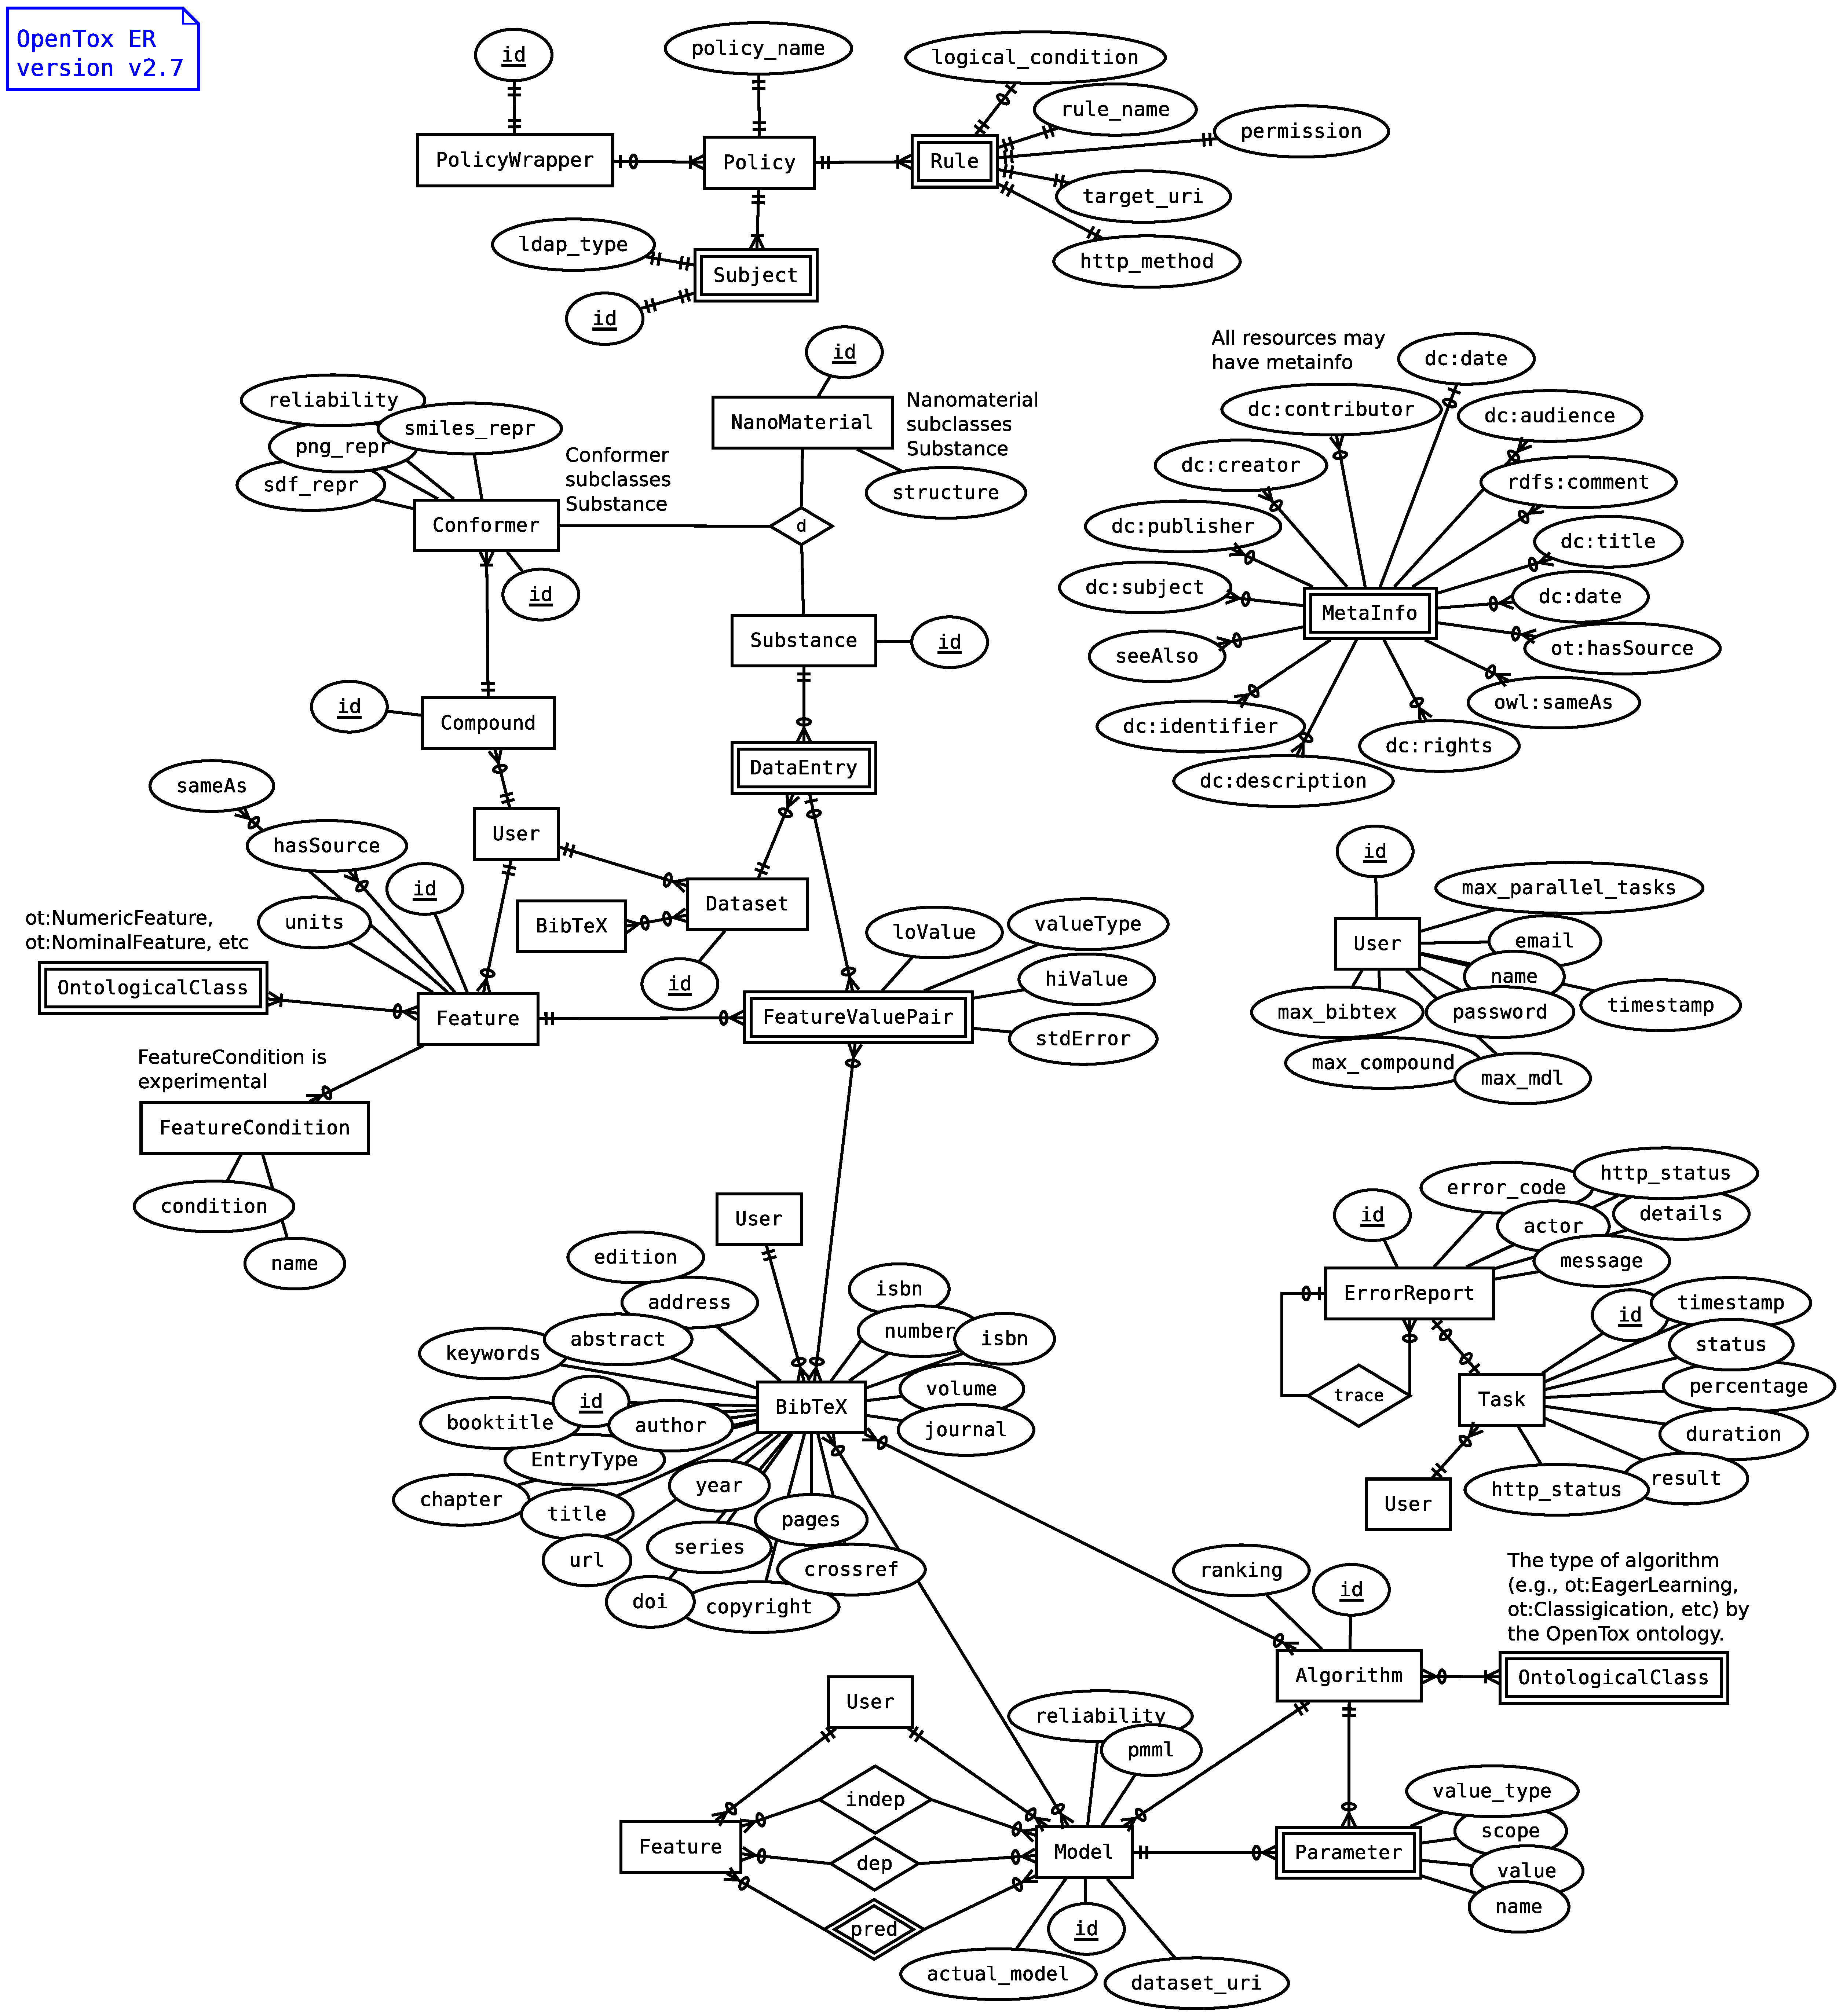
\includegraphics[keepaspectratio=true,width=0.99\textwidth]{figures/er}
\end{figure}

\subsection{Substance}
Substance is a central figure in JAQPOT: A Substance can be either a
chemical Conformer or a Nanomaterial, while in the future other classes
may be added (e.g., proteins, DNA, etc.). A Substance from JAQPOT's
perspective is (i) what identifies a \textit{row} in a \textit{dataset} for
training and (ii) input for prediction using a model.
Substances are abstract entitied. In particular, in the current version, they
are subclassed by the distinct classes \texttt{Nanomaterial} and \texttt{Conformer}.

\subsection{Conformer}
A Conformer is a chemical compound with a particular 3D configuration.
Chemical conformers are groupped together by the same \texttt{Compound}.
Conformers are characterized by their IDs and their various representations
(SMILES, SDF, InChI, etc).

\subsection{Nanomaterials}
A nanomaterial is a particular instance of a Substance. Nanomaterials'
structure is described by the NPO ontology (http://www.nano-ontology.org/).



\subsection{Feature}
Features are properties that can be assigned to substances. The type of
a feature is determined by a link to an ontological class. For instance
a feature can be \texttt{ot:NominalFeature} or \texttt{ot:NumericFeature}
etc. Different features may be groupped together via \texttt{FeatureCondition}s.
Features possess also an ontological characterisation that can be 
used to search for them. When the feature can be computed \textit{in silico}
its \texttt{hasSource} attribute
is a link to the algorithm or model that can be used to compute it.


\subsection{FeatureValuePair}
A \texttt{FeatureValuePair} is exactly what its name implies: 
an feature-value pair in the database
for a particular substance and a given feature.
A Feature value pair may be part of a \texttt{DataEntry} whic is 
the elementary component of a Dataset. This entity has a lower
and a higher bound (in case it is single-valued, by convention,
\texttt{loValue} stores the value and \texttt{hiValue} is set to 
\texttt{null}. It has a value type (numeric, double, integer, 
etc), an error estimation (\textit{e.g.}, \texttt{stdError}).


\subsection{DataEntry and Dataset}
A data entry is simply a \textit{row} in a dataset;
there is a single substance (chemical conformer or nanomaterial) to which
the DataEntry pertains to. A Dataset is chiefly a collection of 
DataEntry entities. 
\section{Querying requirements}



\noindent Here we present a list of queries that one will be expected 
to perform on the DB based on the REST API of OpenTox.

\noindent General remarks:
\begin{enumerate}
 \item Consistency on delete is not an important feature of Jaqpot.
 \item Other comments
\end{enumerate}


\subsection{Tasks and Error Reports}

\noindent Read operations:
\begin{enumerate}
 \item Get task representation by ID
 \item Get a list of task IDs:
    \begin{enumerate}
    \item from a given user
    \item with a given status (\textit{e.g.}, running)
    \end{enumerate}
 \item List all task IDs (paginated)
\end{enumerate}

\noindent Write operations:
\begin{enumerate}
 \item Write new task as \texttt{QUEUED} (default)
 \item Update the meta-data and/or status of a task
\end{enumerate}

\noindent Remarks:
\begin{enumerate}
 \item 	Here we have the most write and read intensive DB 
	operations. Tasks can well be stored in an independent 
	in-memory DB such as Redis. However, this would mean 
	that when we restart the server, all tasks will be lost. 
	Not sure this is the best choice. We can still store the 
	tasks in a document DB (e.g., CouchBase).
 \item 	In case of nested ErrorReport entities, children reports are 
        only fetched with their parents.
\end{enumerate}



\subsection{Model}

\noindent Read operations:
\begin{enumerate}
 \item Retrieve a model: Get model representation (metadata only -- 
       no need to load the actual model) given the ID of the model.
 \item Fetch only the actual model (binary object) but not the metadata. 
 \item List all models of a user
 \item List all models of an algorithm 
 \item List all models for a given keyword (facilitate searching in meta-data)
 \item Combinations of the two above (by user and algorithm)
 \item List all model IDs (paginated)
\end{enumerate}


\noindent Write operations:
\begin{enumerate}
 \item Register new model (all info)
 \item Update model to link to a new BibTeX
 \item Update the meta-data of a model (\textit{e.g.}, new title)
 \item Delete or disable model 
\end{enumerate}


\noindent Remarks:
\begin{enumerate}
 \item In models as well as in other resources, when retrieving data from the 
       DB there will never be the need to fetch the user data (only the ID 
       of the user is OK).
 \item Notice that the actual model (binary) and its metadata are never loaded simultaneously.
 \item In the OpenTox API one finds the method \texttt{GET /model/{id}/independent} 
       (and related methods), but there is not need to create very specialized 
       queries to serve these cases. If the model is stored as a document in the DB, 
       it can be retrieved as a whole and then we can pick only the information we are interested in.
\end{enumerate}





\subsection{User}

\noindent Read operations:
\begin{enumerate}
 \item List all user IDs
 \item Get the representation of a user by ID
 \item Get user's quota (part of the user representation actually)
\end{enumerate}


\noindent Write operations:
\begin{enumerate}
  \item Create new user
  \item Update user quota limits
  \item Delete user
\end{enumerate}



\subsection{BibTeX}

\noindent Read operations:
\begin{enumerate}
\item Get the full representation of a BibTeX entity
\item Search given a keyword
\item List all BibTeX entries
\end{enumerate}

\noindent Write operations:
\begin{enumerate}
 \item Create new BibTeX
 \item Update BibTeX
 \item Delete BibTeX
\end{enumerate}


\noindent Remarks:\\
BibTeX entities have really a lot of fields and it wouldn’t make sense 
to have indexes for every such field. In these cases, we can introduce simply 
a new keyword field that will be indexed and will do the job.


\subsection{Features}
\noindent Read operations
\begin{enumerate}
 \item Get representation of a feature by ID
 \item List features (not too important)
 \item Search features that are sameAs some other feature or feature category (ontology)
 \item Search for features by \texttt{hasSource}
 \item Search for features by their name or some keyword
\end{enumerate}
 

\noindent Write operations
\begin{enumerate}
 \item Create new feature
 \item Update a feature (replace)
 \item Delete feature
\end{enumerate}



\subsection{Compounds}

\noindent Read operations:
\begin{enumerate}
 \item List compound IDs (paginated)
\item  Fetch the representation of a compound ID
\item  Search for the ID of a compound: (i) according to a keyword (we can use ElasticSearch) 
       and/or (ii) the is \texttt{sameAs} some other feature or feature category from an ontology
\item  Fetch a compound along with some features [returns a dataset]. 
   The corresponding API method is \texttt{GET /compound/\{cid\}/feature}
\item  Get all the conformers of a given compound
\end{enumerate}


\noindent Write operations:
\begin{enumerate}
\item Write a new compound in the DB
\item  Update compound
\item  Delete compound
\item  Add conformers to a given compound
\item  Update the representation of a conformer (using PUT)
\end{enumerate}


\noindent Remarks
\begin{enumerate}
\item  It is important to decide whether we will be saving every 
representation of the compound in the database, or whether the new 
representation will be calculated on the fly from what is found in the DB. 
\textit{e.g.}, A client uploads the compound ‘aspirin’ on jaqpot4 in SDF and 
creates a new resource, namely \texttt{/compound/123}. 
Then one needs to retrieve \texttt{/compound/123} is MOL format. 
Will this be generated on the fly? I guess this depends on how fast 
this conversion can be done. 
\item When retrieving datasets from the DB we do not need to 
retrieve any representation of the compound. All compounds appear as links in the dataset.
\end{enumerate}



\subsection{FeatureValuePair}

The only operation that is related to FeatureValuePair entities is the one implied by the API method 
\texttt{POST /compound/\{cid\}/feature?feature\_uri=\{feature\}\& value=\{value\}} 
where a new value is stored in the DB as a FeatureValuePair

\subsection{Dataset}

\noindent Read operations
\begin{enumerate}
 \item Get all dataset IDs (list, paginated)
\item  Fetch a dataset of given ID
\item  List all datasets (IDs) that have a property (\textit{e.g.}, 
   \texttt{created by user x} or \texttt{are annotated as \#jaqpot}). This can be simply done using ElasticSearch!
\item  Get all features and feature values of a given compound (also discussed in Section “Compound”)
\item  Merge datasets
\item  Add compounds to datasets (creates new dataset on the fly)
\item  Fetch a dataset and append a few features
\end{enumerate}


\noindent Write operations
\begin{enumerate}
\item  Create a new dataset (store all its values and the whole structure in the DB)
\item  Update a dataset (replace existing one)
\item Delete a dataset
\end{enumerate}

\noindent Remark: It seems we cannot store datasets in compact documents for many reasons. 
One reason is that whenever a feature-value pair entry is modified, this needs to be known to 
all datasets that use this value. \textit{e.g.}, if a client needs to modify the value of \texttt{molecular mass}
of \texttt{aspirin}, this needs to be updated in all datasets. 
Datasets are therefore collections of DataEntry entities.




\subsection{Algorithm}

There are certain cases that we need to store Algorithm entities
in the DB. Descriptor calculation algorithms (especially when they 
admit input parameters) may need to store new algorithm objects in the database. 
See http://opentox.org/
dev/apis/api-1.2/Algorithm\#section-7 for details. 
Algorithms are simply stored and retrieved as documents. Search is necessary only 
to return those algorithms that are sameAs some ontological category (need for one index). 
In detail we have:

\noindent Read operations
\begin{enumerate}
 \item List all algorithms
\item  Fetch algorithm by ID
\item  List algorithms that are sameAs a given ontological class
\item  List all algorithms generated by a user
\end{enumerate}

\noindent Write operations\\
Register a new algorithm

\subsection{Policy}

\noindent Read operations
\begin{enumerate}
 \item Fetch a policy of a given ID
\item  List all policies of a given user
\item  Search for a policy for a URI (allowed to the owner of the policy only)
\end{enumerate}


\noindent Write operations
\begin{enumerate}
\item  Register policy
\item  Update policy (replace)
\item  Delete policy
\end{enumerate}

\section{Database schema}
JAQPOT Quattro will make use of a document database, 
which is to a good extent schema-less. Here we discuss about 
the basic documents of JAQPOT Quattro and the indexes we need to 
introduce so as to maximize the performance of the 
search, insert and update operations defined previously.

The overall data schema refers to three databases:

\begin{enumerate}
 \item  A document database, in our case mongodb, that stores data in the form of documents. 
 Most of JAQPOT’s resources are stored in this database,
\item  A relational database system, here mysql, that stores certain relations that have to do with datasets
\item  An ElasticSearch DB system that stores keyword-related data to facilitate the exploration of our domain.
\end{enumerate}

\subsection{Task and ErrorReport}

\textit{Example 1.} A completed task (note: duration is in milliseconds).

\begin{lstlisting}[language=json]
{ 
    "status":"COMPLETED", 
    "http_status":200, 
    "result": "http://opentox.ntua.gr:8080/model/234", 
    "duration":452, 
    "progress":[ 
        "data loaded", 
        "new resources have been created", 
        "now training the model", 
        "model training completed", 
        "result: OK" 
        ], 
    "creator":"guest@opentox.ntua.gr", 
    "time_created":"2015-12-01 14:04:45 CET" 
} 
\end{lstlisting}

\noindent \textit{Example 2.} A failed task with an error report in it:
\begin{lstlisting}[language=json]
{ 
    "status":"ERROR", 
    "http_status":400, 
    "duration":200, 
    "progress":[ 
        "data loaded", 
        "new resources have been created", 
        "now training the model", 
        "failed!" 
        ], 
    "creator":"guest@opentox.ntua.gr", 
    "time_created":"2015-12-01 14:04:45 CET", 
    "error_report":{ 
        "error_code":"XR243", 
        "actor":"client with IP 10.8.0.4", 
        "message":"Malformed input data", 
        "details":"Provide some details here to assist debugging", 
        "trace": { 
            "comment":"some other error report goes here if necessary" 
        } 
    } 
} 
\end{lstlisting}

\noindent \textit{Example 3.} A running task:
\begin{lstlisting}[language=json]
{ 
    "status":"RUNNING", 
    "percentage":57, 
    "http_status":202, 
    "progress":[ 
        "data loaded", 
        "new resources have been created", 
        "now training the model" 
        ], 
    "creator":"guest@opentox.ntua.gr", 
    "time_created":"2015-12-01 14:04:45 CET" 
} 
\end{lstlisting}

Notice that we do not assign IDs to the above documents since 
mongodb will create automatically a unique ID which is always 
denoted by \texttt{\_id}.

Indexes:
1. creator
2. status
3. (creator, status)

\begin{lstlisting}[language=json]
db.tasks.ensureIndex({"creator":1});
db.tasks.ensureIndex({"status":1});
db.tasks.ensureIndex({"creator":1, "status":1});
\end{lstlisting}

One can update the metadata of a task. 
See this example:
\begin{lstlisting}[language=json]
db.tasks.update( 
  { _id: ObjectId("54b454f8feee5a13a43f34f3") },  
  { $addToSet:  
     { "progress": "moved to step 4" } 
  } 
); 
\end{lstlisting}

All other update operations can be performed in a very standard way.

It is possible to fetch the data of a document from the DB without the data in a given field. 
For example, we can fetch a task without the progress information 
(here we assume we know the ID of the task):

\begin{lstlisting}[language=json]
db.tasks.find(
  {_id: ObjectId("54b454f8feee5a13a43f34f3")}, 
  {progress:0}
).pretty();
\end{lstlisting}

in some cases we may need to check only the status of a task (provided that we know its ID):
\begin{lstlisting}[language=json]
db.tasks.find(
  {_id: ObjectId("54b454f8feee5a13a43f34f3")}, 
  {status:1}
).pretty();
\end{lstlisting}

Remarks:
\begin{enumerate}
 \item Tasks should be implemented as TTL (time-to-live) collections so that old tasks are garbage-collected.
\end{enumerate}

\subsection{Model}
Example Model document:
\begin{lstlisting}[language=json]
{
    "algorithm":"http://opentox.ntua.gr:8080/algorithm/xyz",
    "description":"Krugerweilderbengeschaft's algorithm",
    "bibtex_ref":"http://opentox.ntua.gr:8080/bibtex/asdf123",
    "creator":"hampos@jaqpot.ntua.gr",
    "actual_model_id":"fsfhafkjaf1234",
    "reliability":2,
    "dataset_uri":"http://opentox.ntua.gr:8080/dataset/5432",
    "independent_features":[H
        "http://someserver.org:1234/feature/1",
        "http://someserver.org:1234/feature/2",
        "http://someserver.org:1234/feature/3",
        "http://someserver.org:1234/feature/4",
        "http://someserver.org:1234/feature/5"
    ],
    "dependent_feature":"http://otherserver.org:1234/feature/100",
    "predicted_feature":"http://otherserver.org:1234/feature/455",
    "parameters":[
        {
            "name":"alpha",
            "value":14,
            "scope":"mandatory",
            "value_type":"numeric",
            "description":"convergence rate"
        },
        {
            "name":"tolerance",
            "value":0.004,
            "scope":"optional",
            "value_type":"numeric"
        }
    ]
}
\end{lstlisting}

\noindent Indexes:
\begin{enumerate}
 \item creator
\item algorithm
\item (creator, algorithm)
\end{enumerate}

The actual model of a Model are stored outside the model document.  
Note that when the metadata of the model are requested (when the method 
\texttt{GET /model/\{id\}} is invoked), the actual (binary) model 
data are not fetched.


\subsection{User}
Here is an example of a user (note: passwords are hashed):
\begin{lstlisting}[language=json]
{ 
  "uid":"guest@opentox.ntua.gr", 
  "name":"Guest Guestopoulos", 
  "timestamp":"2015-01-01 15:08:01 CET", 
  "password":"SDF#YHFDJSNF5443#*@RY", 
  "email":"guest@guest.org", 
  "max_models":10000, 
  "max_bibtex":-1, 
  "max_compounds":50000, 
  "max_parallel_tasks":5 
} 
\end{lstlisting}
the read operations we require are very simple: search by \texttt{\_id}, 
update the quota limits, delete a user.

\subsection{BibTeX}
Most entries of a BibTeX entity need to be searchable; 
therefore, we introduce them into an ElasticSearch database. 
The same concept will be used also for other cases where we need advanced 
search capabilities. The ElasticSearch DB will return the IDs of the 
BibTeX entries that match a given query so that the actual data can then 
be retrieved from the mongodb database, that is ElasticSearch is used to 
retrieve indices very fast and very efficiently. 

Here is a simple BibTeX document:

\begin{lstlisting}[language=json]
{
    "entry_type":"article",
    "bibtex_key":"MayRaw+00",
    "title":"Constrained model predictive control: Stability and optimality",
    "author":"D.Q. Mayne and J.B. Rawlings and C.V. Rao and P.O.M. Scokaert",
    "journal":"Automatica",
    "volume":36,
    "number":6,
    "pages":"789-814",
    "creator":"chung@jaqpot.org",
    "issn":"0005-1098",
    "doi":"http://dx.doi.org/10.1016/S0005-1098(99)00214-9",   
    "url":"http://www.sciencedirect.com/science/article/pii/S0005109899002149",
    "year":2000,
    "abstract":"Model predictive control is a form of ",
    "pdf":"~/Documents/articles/mpc_paper.pdf",
    "keywords": [
"MPC", 
"Model predictive control",
"Lyapunov theory",
"positive invariance"
    ]
}
\end{lstlisting}
In order to create a new BibTeX entry on ElasticSearch we PUT the above document 
at \texttt{/bibtex/entry/\{bibid\}}, where \texttt{\{bibid\}} is a unique 
identifier of the document. ElasticSearch responds with the following document:
\begin{lstlisting}[language=json]
{
  "_index":"bibtex",
  "_type":"entry",
  "_id":"MayRaw00",
  "_version":1,
  "created":true
}
\end{lstlisting}
%
%
and we can therefore tell that no previously existing document has been replaced. 
We can of course use POST for an ID to be automatically created, but we'll go for 
\texttt{PUT} since in our approach it is Jaqpot Quattor that decides the ID. 
This document can then be found where we put it (if we know its \texttt{\{bibid\}}):

At \texttt{/bibtex/entry/MayRaw00}, we retrieve the following document:
\begin{lstlisting}[language=json]
{ 
  "_index" : "bibtex", 
  "_type" : "entry", 
  "_id" : "MayRaw00", 
  "_version" : 6, 
  "found" : true, 
  "_source": 
{ 
    "entry_type":"article", 
    "bibtex_key":"MayRaw+00", 
    "title":"Constrained model predictive control: Stability and optimality", 
    "author":"D.Q. Mayne and J.B. Rawlings and C.V. Rao and P.O.M. Scokaert", 
    "journal":"Automatica", 
    "volume":36, 
    "number":6, 
    "pages":"789-814", 
    "creator":"chung@jaqpot.org", 
    "issn":"0005-1098", 
    "doi":"http://dx.doi.org/10.1016/S0005-1098(99)00214-9",    
    "url":"http://www.sciencedirect.com/science/article/pii/S0005109899002149", 
    "year":2000, 
    "abstract":"Model predictive control is a form of ", 
    "pdf":"~/Documents/articles/mpc_paper.pdf", 
    "keywords": [ 
"MPC",  
"Model predictive control", 
"Lyapunov theory", 
"positive invariance" 
    ] 
} 
} 
\end{lstlisting}
%
%
A simple query in the database is the following: Find all documents with author ‘Mayne’ (we don’t need to specify all authors):
%
\begin{lstlisting}[language=json]
curl-X GET "localhost:9200/bibtex/entry/_search?q=author:Mayne"
\end{lstlisting}
This returns the response:
\begin{lstlisting}[language=json]
{ 
  "took" : 14, 
  "timed_out" : false, 
  "_shards" : { 
    "total" : 5, 
    "successful" : 5, 
    "failed" : 0 
  }, 
  "hits" : { 
    "total" : 3, 
    "max_score" : 0.25, 
    "hits" : [ { 
      "_index" : "bibtex", 
      "_type" : "entry", 
      "_id" : "MayRaw00", 
      "_score" : 0.25, 
      "_source": 
{ 
    "entry_type":"article", 
    "bibtex_key":"MayRaw+00", 
 [more...]
\end{lstlisting}
%
%
A lot of similar queries can be performed and ElasticSearch has a lot of nice 
features such as \textit{percolation}, \textit{search suggesters}, \textit{more-like-this} features, 
\textit{aggregations} and many more.






\subsection{Feature}
Very simple documents as follows:
\begin{lstlisting}[language=json]
{
    "name":"molecular weight",
    "units":"Da",
    "description":"blah blah",
    "hasSou rce":"http://jaqpot.org:8080/model/45",
    "sourceType":"model",
    "sameAs":"http://someontology.org/v/1.1#MolecularWeight",
    "creator":"chung@jaqpot.org",
    "featureType":"numeric"
}
\end{lstlisting}
%
%
Indexes:
\begin{enumerate}
 \item hasSource
\item  sameAs
\item  creator
\item  possibly combinations of the above
\end{enumerate}


\subsection{Conformers}
A conformer document in JSON looks something like this 
(we will explain why we have adopted this structure, just for 
now remember that the shallower the documents are, the more 
efficient search operations are in document databases):
\begin{lstlisting}[language=json]
{ 
    "father_compound": 55, 
    "name": ["aspirin", "acetylsalicylic acid"], 
    "smiles": "CC(=O)Oc1ccccc1C(=O)O", 
    "inchi_key": "BSYNRYMUTXBXSQ-UHFFFAOYSA-N", 
    "sdf_representation": "http://server.com/compound/2/sdf", 
    "comment": [ 
        "this is a comment", 
        "analogue of rdfs:comment" 
    ], 
    "identifier": "http://opentox.ntua.gr:8080/compound/55/conformer/2", 
    "feature/10":{"title":"average_mass", "value":180.157, "units":"Da"}, 
    "feature/83":{"title":"monoisotropic_mass","value":180.042, "units":"Da"}, 
    "feature/62":{"title":"iupac_name", "value":"2-Acetoxybenzoic acid"} 
} 
\end{lstlisting}
Notice that we can find in the representation of the conformer a 
link to its father (the compound that holds it). Additionally, it is 
not important to have the units of features inside the document, but 
it is of course possible to add them. In the conformer document we can, 
but we do not intend to store data related to prediction features or 
in any other way data that can make the conformer document increase 
endlessly and break the efficiency of our schema. Prediction features 
are stored in a different way (that combines mongodb with a relational 
database system) and the adopted schema is described in the next section.
%
We can easily append some new FeatureValuePair entity like this:

\begin{lstlisting}[language=json] 
db.compounds.update(
    {"_id" : ObjectId("54b46dedee9871fd62716680")}, 
    { $set: 
        { 
          "feature/32": 
              { 
                "title":"CASRN", 
                "value":"50-78-2"
                "description":"CAS registry number"
              } 
        } 
    }
);
\end{lstlisting}

we can also delete such FeatureValuePair entries. One can do many other things such as add tags to the document using 
\texttt{\$addToSet}. Here is a snippet:

\begin{lstlisting}[language=json]
db.compounds.update(  
    {"_id" : ObjectId("54b46dedee9871fd62716680")},  
    { $addToSet:  
        { "tags":"anti-inflammatory" }  
    }  
); 
\end{lstlisting}

It will be necessary to retrieve only some of the fields of a conformer document. Here is how it can work:

\begin{lstlisting}[language=json]
db.compounds.find(
    {"_id" : ObjectId("54b46dedee9871fd62716680")},
    {
      "feature/10":1, 
      "feature/62":1,
      "father_compound":1
    }
);
\end{lstlisting}

this is good practice according to the mongodb online guide which states that "When you need only a subset of fields from documents, you can achieve better performance by returning only the fields you need". The above command will give the following output:
\begin{lstlisting}[language=json]
{
	"_id" : ObjectId("54b46dedee9871fd62716680"),
	"father_compound" : 55,
	"feature/10" : {
		"title" : "average_mass",
		"value" : 180.157
	},
	"feature/62" : {
		"title" : "iupac_name",
		"value" : "2-Acetoxybenzoic acid"
	}
}
\end{lstlisting}

Remarks: 
1. When constructing a dataset we need exactly the following things: conformer links, feature links, and feature-value pairs for each compound. We don’t  need to retrieve the compound representation (SMILES, SDF or any other), or details about the feature or anything else. In simple words: the dataset is expected to deliver the information that can be found in an ARFF document. 
2. We can serialise datasets in SDF format (i.e., a document format that includes the representations of all compounds as well), and this is perfectly feasible in the above context.
3. It may be expedient to introduce an array in Conformer entities that holds all features, i.e., something like:
\begin{lstlisting}[language=json]
{
 "features": [ "feature/14", "feature/15", "feature/16" ] 
}
\end{lstlisting}
For easier and faster lookup. However, these queries don't need to served at maximum efficiency

Important remark: One would have possibly expected a more rational JSON schema in regard to the representation of FeatureValuePair entities, such as the following:

\begin{lstlisting}[language=json]
{ 
    "father_compound": 55, 
    "name": "aspirin", 
    "smiles": "CC(=O)Oc1ccccc1C(=O)O", 
    "inchi_key": "BSYNRYMUTXBXSQ-UHFFFAOYSA-N", 
    "sdf_representation": "http://server.com/compound/2/sdf", 
    "comment": [ 
        "this is a comment", 
        "analogue of rdfs:comment" 
    ], 
    "identifier": "http://opentox.ntua.gr:8080/compound/55/conformer/2", 
    "feature_value_pairs": [ 
        { 
            "feature_name": "average_mass", 
            "feature_id": 10, 
            "comment": [ 
                "feature uri is http://jaqpot.org:8080/feature/10", 
                "this is a FeatureValuePair thing" 
            ], 
            "value": 180.157, 
            "units": "Da" 
        }, 
        { 
            "feature_name": "monoisotropic_mass", 
            "feature_id": 83, 
            "value": 180.042252, 
            "units": "Da", 
            "feature_same_as": "ot:MonoIsoMass" 
        }, 
        { 
            "feature_name": "iupac_name", 
            "feature_id": 62, 
            "value": "2-Acetoxybenzoic acid", 
            "units": "", 
            "feature_same_as":"http://www.opentox.org/api/1.1#ChemicalName"

        } 
    ] 
} 
\end{lstlisting}

However, it is more difficult (yet possible\footnote{Using aggregation (e.g., map-reduce) -- 
see http://docs.mongodb.org/manual/core/aggregation-introduction}) to retrieve from the database a 
filtered document with only some selected feature values. We, therefore, have 
chosen to abide by the principle of shallow documents.

Conformer Lookup: We shall need to be able to lookup for conformers given their
name (each conformer has multiple names, including the IUPAC standard name), or 
SMILES. Features like: ``did you mean...'' or ``type completion'' will also be necessary. 
This is why we shall introduce these fields (name, IUPAC name, smiles) into the ElasticSearch database.

\subsection{Substructual lookups}
Given a SMILES string\footnote{ If the substructure is given in any other representaiton 
(\textit{e.g.}, SDF), it will be first converted to SMILES by JAQPOT.}, we need a very efficient 
way to determine those conformers whose this is a substructure. To this end, we need to 
store for each compound a close-to-complete list of its substructures (mind that for large 
compounds they can be up to some thousands). At the same time, it will also be useful to 
have quick access to the list of substructures of a given compound. For that, we propose 
the following schema:

We extend the aforementioned Conformer schema to include 
these substructures as an array under the field substructures%
\footnote{TBD: there may be more efficient algorithms one may consider (todo: check the literature).}:
\begin{lstlisting}[language=json]
{   "father_compound": 55, 
    "name": "aspirin", 
    "smiles": "CC(=O)Oc1ccccc1C(=O)O",
    "substructures": [ 
	"c1ccccc1", "C", "CC", "CCC", "CCCCCC", "CC(=O)O", "C(=O)O" 
    ],
...
}
\end{lstlisting}

we then also store these substructures in ElasticSearch as follows:
\begin{lstlisting}[language=json]
{ "conformer_id": 56123a42c134edad2342c, 
  "father_id": 55,
  "substructures": ["c1ccccc1", "C", "CC", "CCC", "CCCCCC", "CC(=O)O", "C(=O)O"]
}
\end{lstlisting}

\subsection{Compounds}
Compounds are collections of conformers. Their representation is very simple:
\begin{lstlisting}[language=json]
{ 
    "conformers": [   
      423, 35423, 123, 9130, 9091, 23, 24, 25, 26 
    ]
}
\end{lstlisting}

They are rarely updated and their updates are very easy using \texttt{\$addToSet}.

\subsection{Prediction Feature Data}
Prediction feature data (values) are stored in simple 
documents in the database that look like this:

\begin{lstlisting}[language=json]
{ 
    "_id": ObjectId("54b46dedee9871fd62716680"),
    "feature":"feature/4234524", 
    "value":0.1343,
    "value_type":"numeric"
} 
\end{lstlisting}

a possible query is to ask for a collection of feature values which, in mongodb, is done as follows:
\begin{lstlisting}[language=json]
db.pred.find( 
    {feature:  
        {$in: ["feature/183", "feature/9983"]} 
    } 
).pretty(); 
\end{lstlisting}

a relational database stores the feature-value pair \texttt{\_id} of those 
feature-value pairs that correspond to the predicted features of a dataset. 

\subsection{Datasets}
Datasets are not stored as documents (save cached datasets), but are a set of relations. In particular:
Many datasets have zero-or-many prediction features and zero-or-many conformers and zero-or-many 
prediction feature values (points to document db).
It is then easy to see that the most well-fit structure for our mysql DB is:

\begin{figure}[h]
 \centering
 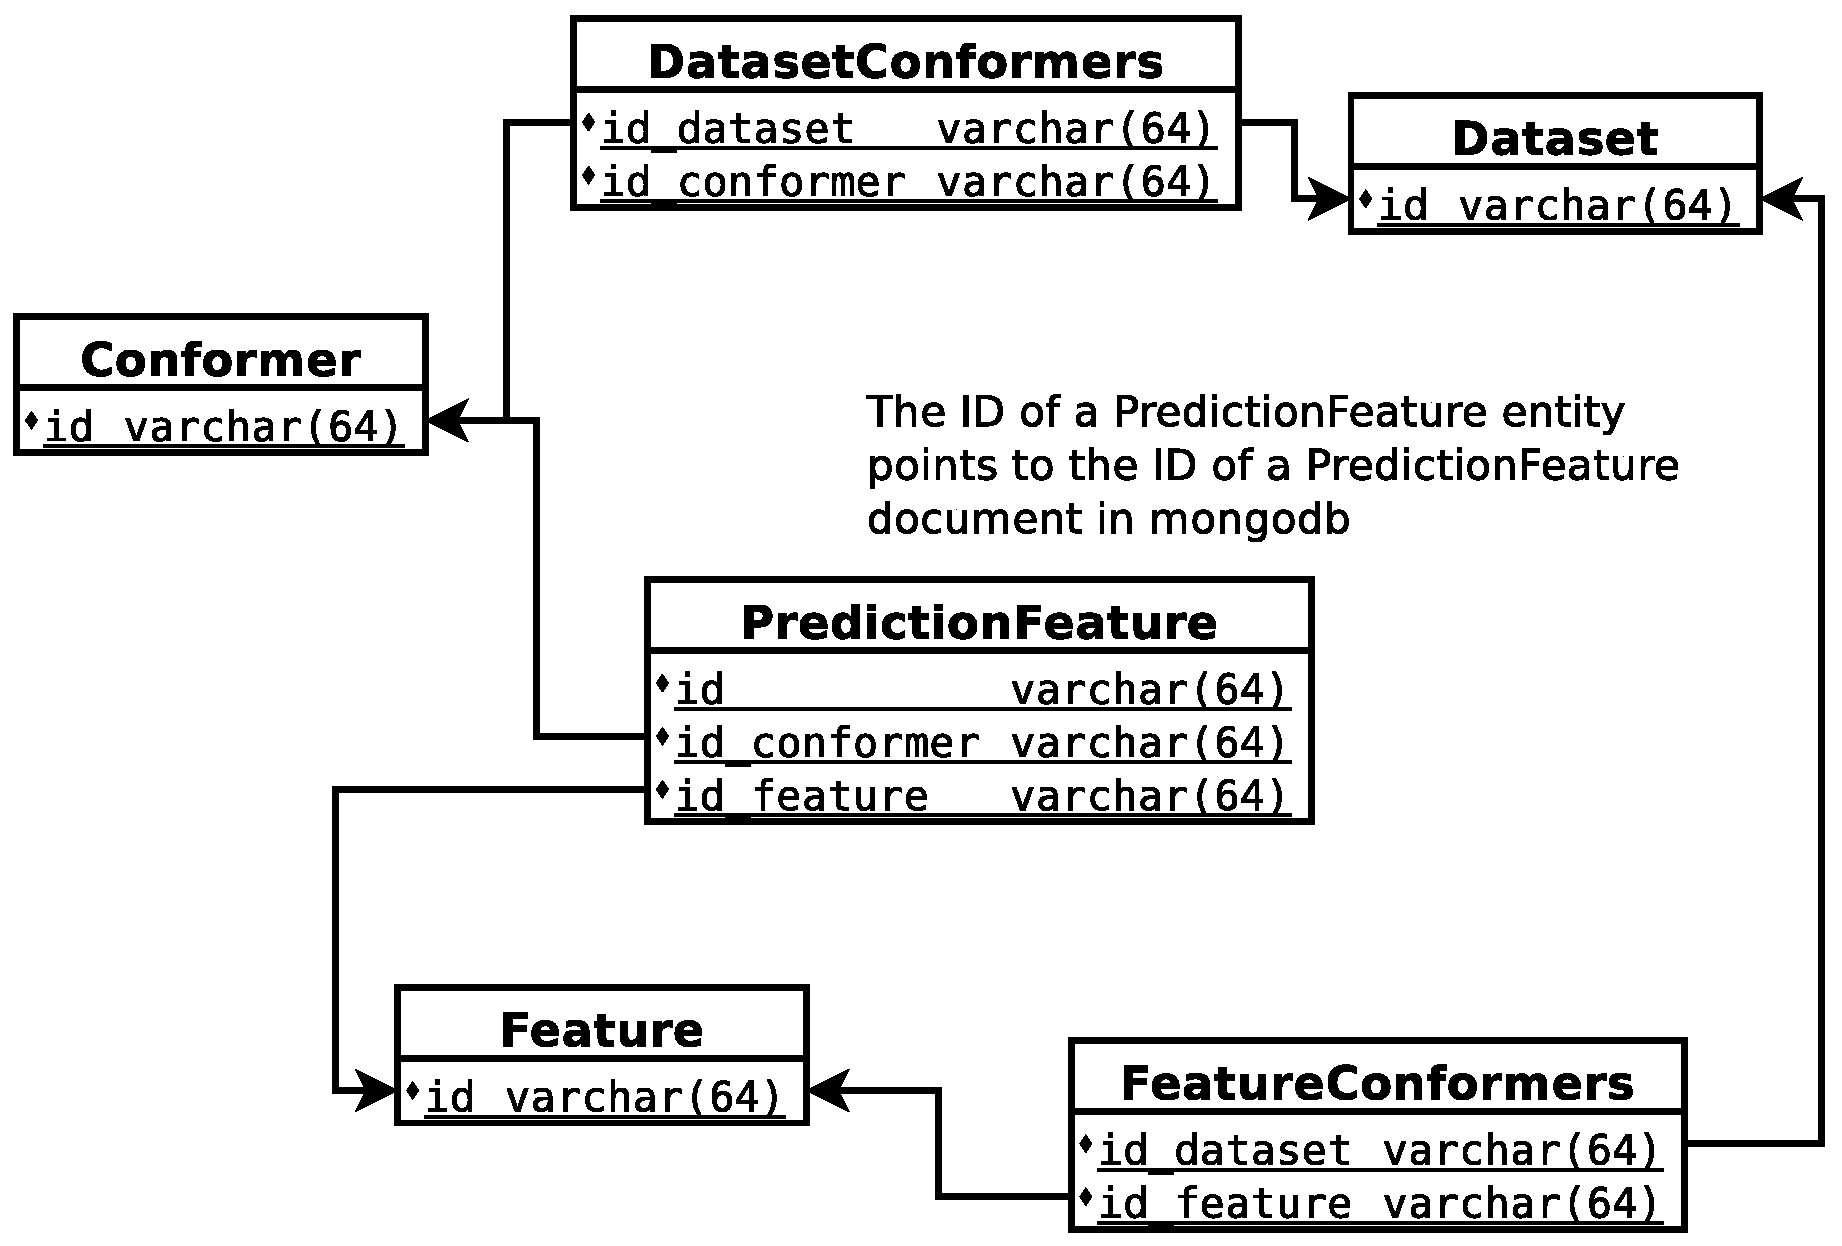
\includegraphics[keepaspectratio=true,width=0.85\textwidth]{figures/JAQPOT_Quattro_RDB}
\end{figure}


Cached Datasets
A MFU cache is employed to store the most frequently used dataset objects. On top of our implementation, mongodb will keep in RAM some of them.

\subsection{Algorithm}


\subsection{Policies and Authentication Tokens}
A policy infrastructure can be implemented extending the current API 
(based on SSO). This can be a general purpose A\&A infrastructure running separately 
and independently of JAQPOT. A policy specifies access-rules method-wise. 
Here is a representation of a JAQPOT4 policy:
\begin{lstlisting}[language=json]
{
  "policy_name":""model_eaa7f89f",
  "creator":"chung@jaqpot.org",
  "creation_date":"1413354887912",
  "last_modified":"1413354887912",
  "target":"http://jaqpot.org/model/123",
  "rules": [
    {
    "allowed_methods": ["get", "post"],
    "subject_type":"user",
    "subjects": [
      "user1@jaqpot.org",
      "user2@jaqpot.org"
    ]
    },
    {
    "allowed_methods": ["get","post","put","delete"],
    "subject_type":"group",
    "subjects": [ "group:admins" ]
    }
  ]
}
\end{lstlisting}

Rules are by default non-exclusive; if a rule allows a subject to apply the method, 
then permission is finally granted to them. This can be overriden by specifying a 
propositional logic equivalence between rules. In the example above for instance, 
say user \texttt{user1@jaqpot.org} is an administrator. Then the first rule doesn't 
allow the user to apply a put, but the second one does; at the end of the day, the user 
must be granted access. 

\chapter{JPDI Architecture}
Jaqpot Protocol of Data Interchange, shortly JPDI, 
is a brand new feature of JAQPOT that allows developers 
of QSAR-related or machine learning algorithms to 
integrate their implementations in JAQPOT so that these
can be used by JAQPOT for QSAR.


n Jaqpot3 a Dataset is frequently consumed in ARFF format by the Dataset service, 
as Weka is the main QSAR engine and Weka Instances can easily be created by ARFF. 
Then all pre-processing is done on those Instances and the Algorithm training as well. 
ARFF and Instances are quite convenient when applying Weka algorithms on a Dataset, 
but not a generic solution to accommodate different Algorithmic engines.
 
Jaqpot Quattro introduces OpenCPU, an HTTP proxy to R, a language that has 
interesting packages regarding QSAR. In order to interact with R, Jaqpot must consume an 
OpenCPU resource that masks an R function and provide a Dataset in Json format as input 
to that function. The input Dataset could also be enriched by some extra detail, as to 
which of the Features is to be predicted, and various parameters if 
needed by the specific algorithm.


\section{JPDI Specification}
Algorithm implementation could be decoupled from Jaqpot. 
Taking example from the OpenCPU solution, we could create different 
individual services for each QSAR engine and it’s algorithms. Then a user could 
use Jaqpot's Algorithm service to create/update/remove Algorithm resources at will. 

\begin{figure}[h]
 \centering
 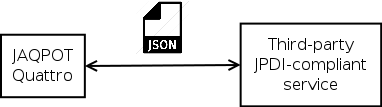
\includegraphics[keepaspectratio=true,width=0.6\textwidth]{figures/JPDI_general.png}
\end{figure}

As shown in the above figure, JAQPOT communicates with 
third-party, external, and independent WSs over HTTP
using a very simple REST interface that we will discuss
hereafter and uses JSON as the standard data exchange format.
The essential principles of JPDI are the following:


\begin{enumerate}
 \item The JPDI API is super-easy for non-expert programmers to 
 implement (so that people can get to integrate their algorithms in
 JAQPOT); JPDI compliant services do not need to maintain a database
 or implement a queue of asynchronous jobs\footnote{this would be
 required for someone to implement an OpenTox-compliant WS, but building
 a JPDI-compliant WS is piece of cake!},
 \item JAQPOT and JPDI services are developed independently,
 \item Services communicate over HTTP exchanging JSON files
 \item Services exchange only what is necessary in the way the JPDI
 specs mandate,
 \item Integration is seamless: JPDI services are plug-in, plug-out 
 and can be added or removed from JAQPOT Quattro at any time,
 \item Third-party services are absolutely free to decide how they
 want to store their models on JAQPOT (the can store them even in 
 custom binary formats).
\end{enumerate}


\section{Training with JPDI-compliant WSs}
Training with a JPDI-compliant WS is explained in this section.
As we see in the following picture, the JAQPOT User Interface 
in collaboration with the JAQPOT Web Services prepares all necessary
data to be sent to the JPDI training service. The following input is
provided to the training service:

\begin{enumerate}
 \item The training dataset where the target feature is 
 indicated to the training service, 
 \item tuning parameters of the algorithm as requested by JPDI
 \item other metadata that \textit{may} be useful to the JPDI service
 (\textit{e.g.}, the URI of the training dataset).
\end{enumerate}
\begin{figure}
\centering
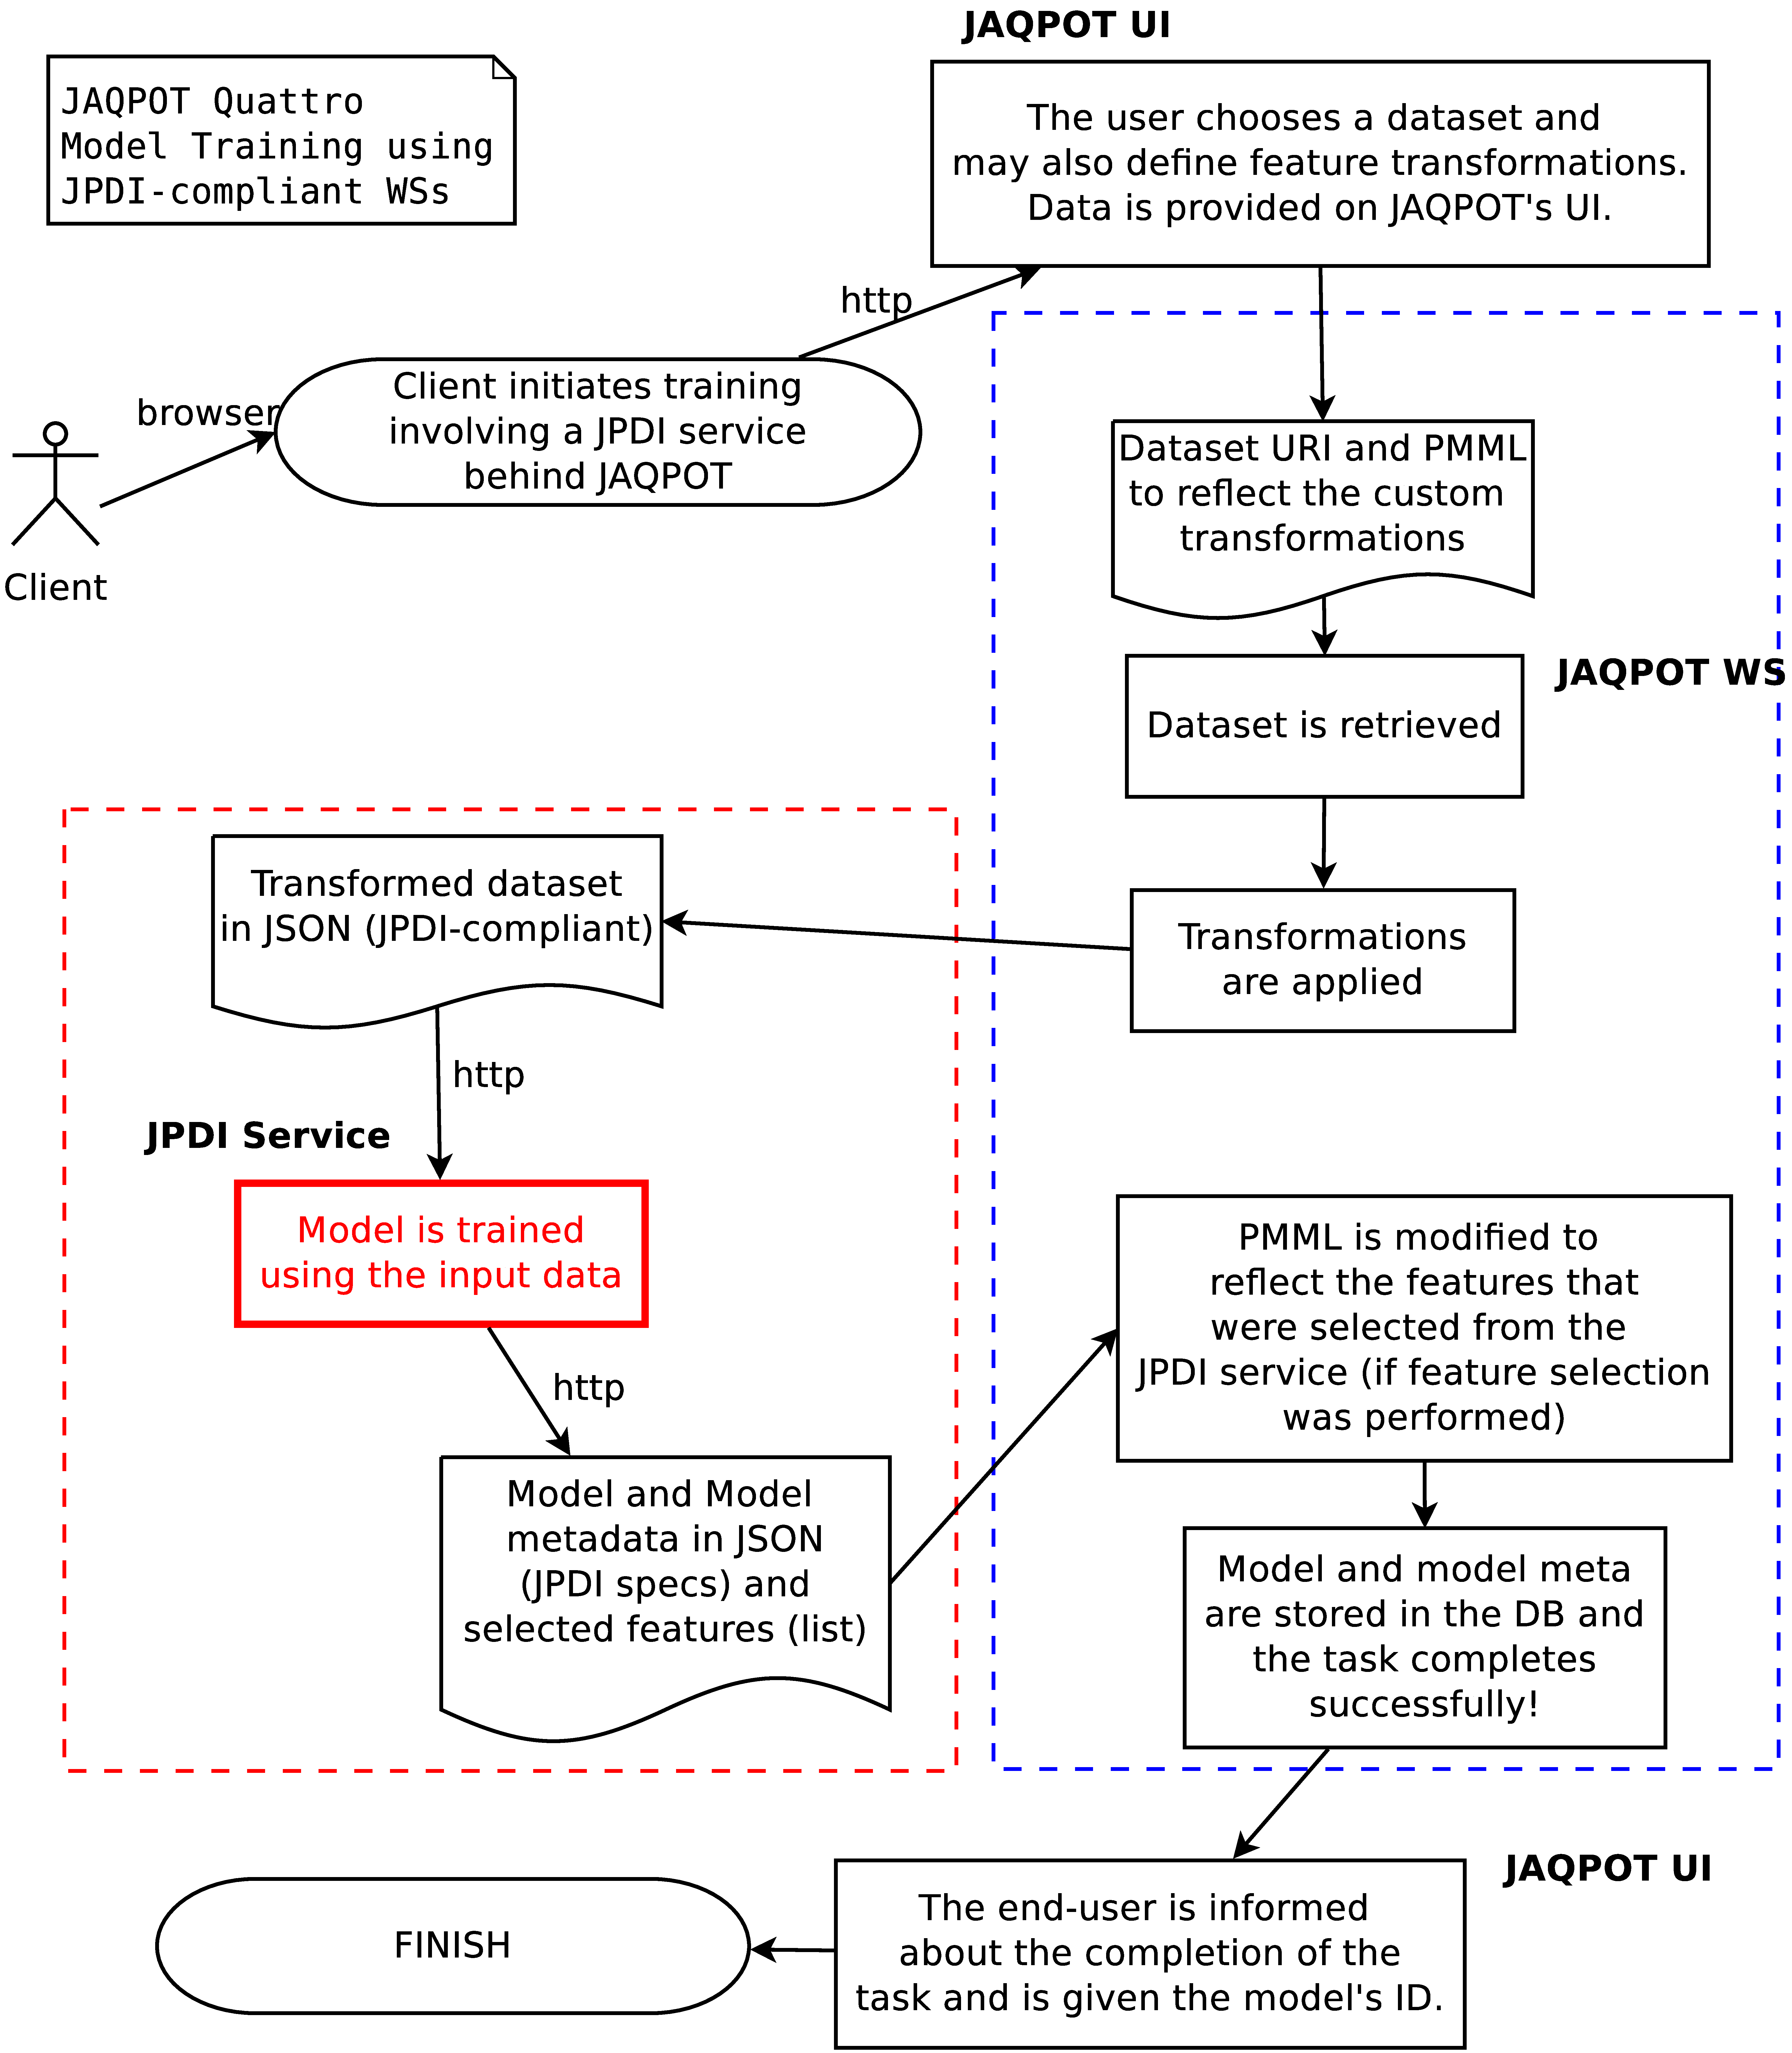
\includegraphics[keepaspectratio=true,width=0.999\textwidth]{figures/JPDI_training.eps}
\end{figure}
Here is an example of a training request in JSON. 
A training service has all that it needs to train a
new machine-learning model. Notice that missing values are set
to \texttt{null}.
Algorithm-specific parameters are passed to the training service
in the same JSON documents.

\begin{lstlisting}[language=json]
 {
    "jpdi_verion" : "1.0.0",
    "data" : {
      "/compound/1/conformer/11": 
	  [1.23, 2.44, 5.01, null, 0.07, 0.94],
      "/compound/2/conformer/31": 
	  [9.31, 1.90, 8.11, 0.05, 0.21, 0.88],
      "/compound/3/conformer/90": 
	  [8.10, 0.67, 7.10, 0.00, 0.44, 0.67],
      "/compound/4/conformer/45": 
	  [3.91, 1.03, 8.37, 0.28, null, 0.99]
    },
    "parameters" : {
      "lambda" : 1,
      "c" : 0.8,
      "epsilon" : 0.1,
      "tolerance" : 0.00001
    }
}
\end{lstlisting}

The, the JPDI service will process this information and will
produce a model that can be stored in any format (this is to 
be decided by the JPDI service developers). We suggest PMML 
if it is possible that the model can be serialized in this 
format. If the model is to be serialized in some custom binary
format we recommend that it is encoded in \texttt{Base91} (although,
it is completely up to the service provider to decide that).


Once the model is trained, the JPDI service will return it
to JAQPOT in JSON in which the actual model is encoded.
Here is an example:

\begin{lstlisting}[language=json]
{
  "feature_selection": true,
  "selected_features" : [1, 2, 5],
  "model":"FSKHEKJFBADNFBDABDABSD..."
} 
\end{lstlisting}

The actual model data is stored under \texttt{model}; of course
JAQPOT cannot interpret this data, so the JPDI service is also 
responsible to provide predictions when a user needs to use 
the model. Notice that here the JPDI service also performed 
feature selection and selected the first, the 
second and the fifth features among the ones that were given to it%
\footnote{The JPDI service doesn't (need to) know what the input features
really are, so their URIs are useless to it. Likewise, it can perform
feature selection without having access to the feature definitions/metadata.
The take-away message is that JPDI training services do \textbf{only} training.}.
Now this model is stored in the DB of JAQPOT and a new model resource is created
and is assigned a new URI.

In this example of model training, since the training
WS has selected these 3 features as input features, 
when one needs to do a prediction, these exact features 
in this very order need to be sent to the JPDI service.
This is done in a very easy way as we see in the training 
workflow: the PMML file is modified to store the necessary
feature transformations and feature selection so as to
create a dataset for prediction.



\section{Prediction with JPDI-compliant WSs}


\section{Registration of new algorithms}
New algorithms need to be \textit{registered} on JAQPOT Quattro
so that JAQPOT knows how to invoke them. This is specified in 
a very simple manner on registration. JPDI algorithms
are registered by a POST method applied on \texttt{/algorithm}
specifying with a JSON document the following:
\begin{enumerate}
 \item Metadata of the algorithm such as its title, description,
 authors, link(s) to BibTeX entry(ies), comments, a copyright notice,
 contributors, and more,
 \item The type of the algorithms according to the OpenTox algorithm
 ontology (e.g., EagerLearning, Regression),
 \item A list of parameters of the algorithm (both mandatory and optional).
 A parameter of an algorithm has a name, a description (possible also more
 metadata if necessary), a type (numeric/binary/string etc), and
 a scope (optional/mandatory).
\end{enumerate}
Below, we give an example of an algorithm registration request.

\begin{lstlisting}[language=json]
{
  "title": "SuperTraining",
  "description" : "this is a mighty algorithm",
  "author" : "W.Y. Chung",
  "algorithmTypes" : ["EagerLearning", "Regression"],
  "parameters": [
    {
      "name" : "x",
      "description" : "this is x",
      "default_value" : 0.045,
      "type" : "numeric",
      "scope" : "optional"
    },
    {
      "name" : "y",
      "description" : "this is y",
      "default_value" : true,
      "type" : "boolean",
      "scope" : "optional"
    },
  ]
} 
\end{lstlisting}

JAQPOT then responds with the URI of the algorithm that 
was created (if the request succeeds) in \texttt{text/uri-list}.

\section{Access restriction}
When a user creates a new algorithm (following the procedure described here
above), access is granted only to them only. Users can then modify the access
policy on their algorithm to grant access to other users or even make 
these algorithms publicly accessible. Algorithms will receive ranking
from users. Until an algorithm reaches high ranking, or is approved by
the administrators of JAQPOT, it will be tagged as \textit{experimental}.
\chapter{Datasets from Studies}

\section{Introduction}
JAQPOT Quattro is a essentially a QSAR model training/prediction software and, 
as such, it should accept a properly formed dataset as input to all 
such calculations. In old OpenTox times, the standard process of training 
and prediction was as follows (short overview of what we already know):\\\\

\noindent Training flow:
\begin{enumerate}
 \item 	User consumes a Jaqpot algorithm resource and provides a 
	specific Dataset from a Dataset service. Also selects a feature to be 
	predicted. (Optionally provides a PMML file to specify a multitude of 
	transformations to be applied to the dataset before training)
\item  Jaqpot responds to the user with a created Task for the required procedure.
\item   Jaqpot downloads the dataset in a properly formed manner.
 \item  Jaqpot does preprocessing on the dataset, as dictated by the algorithm and/or the PMML file the user provided.
 \item  Jaqpot applies the selected algorithm on the dataset (excluding the prediction feature) and trains a Model. 
 \item  Jaqpot creates a new Feature in a Feature service in order to store the results of the Model when the latter is to be used for training purposes. The URI of that new Feature is saved in the Model.
 \item  Jaqpot persists the model in the database and injects a new URI created for that model in the procedure’s Task.
 \item  User consumes the given Task to acquire the URI of the created Model.
\end{enumerate}

 
 
 
\noindent Prediction:
\begin{enumerate}
\item  User consumes a Jaqpot Model resource and provides a specific Dataset from a Dataset service, and a Dataset Service on which the prediction should be made. (Optionally provides a PMML file to specify a multitude of transformations to be applied to the dataset before prediction)
\item Jaqpot responds to the user with a created Task for the required procedure.
\item Jaqpot downloads the dataset in a properly formed manner.
\item Jaqpot does preprocessing on the dataset, as dictated by the model’s algorithm and/or the PMML file the user provided.
\item Jaqpot applies the selected model on the dataset and creates an array of predicted values.
\item Jaqpot creates a new dataset by adding the array of predicted values on the original dataset. (adding a new Feature column with the URI of the Feature the model has saved for prediction purposes.)
\item Jaqpot saves the newly created Dataset to the Dataset Service the user specified for prediction purposes (could very well be the same service with the original Dataset), and injects the URI of the new Dataset in the procedure’s Task.
\item User consumes the given Task to acquire the URI of the created Dataset.
\end{enumerate}

These old procedures are very straightforward and intuitive and its pretty 
obvious that no user interaction is needed in any steps between the first 
and the last step of each procedure. Alas, changes must be made to allow 
collaboration into the new eNM mindset.


In eNanoMapper, construction of a properly formed Dataset by experimental 
data of engineered nano-materials is not a trivial matter and should not be 
confronted as such. Each Substance does not have a finite domain of Features, 
as in Compounds and Conformers. What it does have is a collection of Studies, 
each one with multiple measurements concerning a single experiment. 

A reference URI for a collection of studies in a Substance: 

https://apps.ideaconsult.net/enmtest/substance/FCSV-b87fcc13-ef28-3edb-9049-3153303b8076/study?media=application\%2Fjson



\end{document}